\textbf{Security aspects of communication model.} We would like to start our thesis with a general description of the
communication structure between an actors among with possible security and user privacy vulnerabilities.
Communication model of the instant messaging system is a quite large topic since it implies various protocols, approaches etc,
therefore current discussion asserts the communication over HTTP protocol via REST API\@ using JSON data format.
Since that main task of this thesis is to implement software components that meet the specified security requirements,
namely: \textit{Web Client, Web API (Application Programming Interface), Mobile client, Desktop client} which are
considered to be the actors we focus our attention to.
The following diagram describes the basic concept of the system, and conveys the relationships between the actors mentioned above.

\begin{figure}[H]
    \centering
    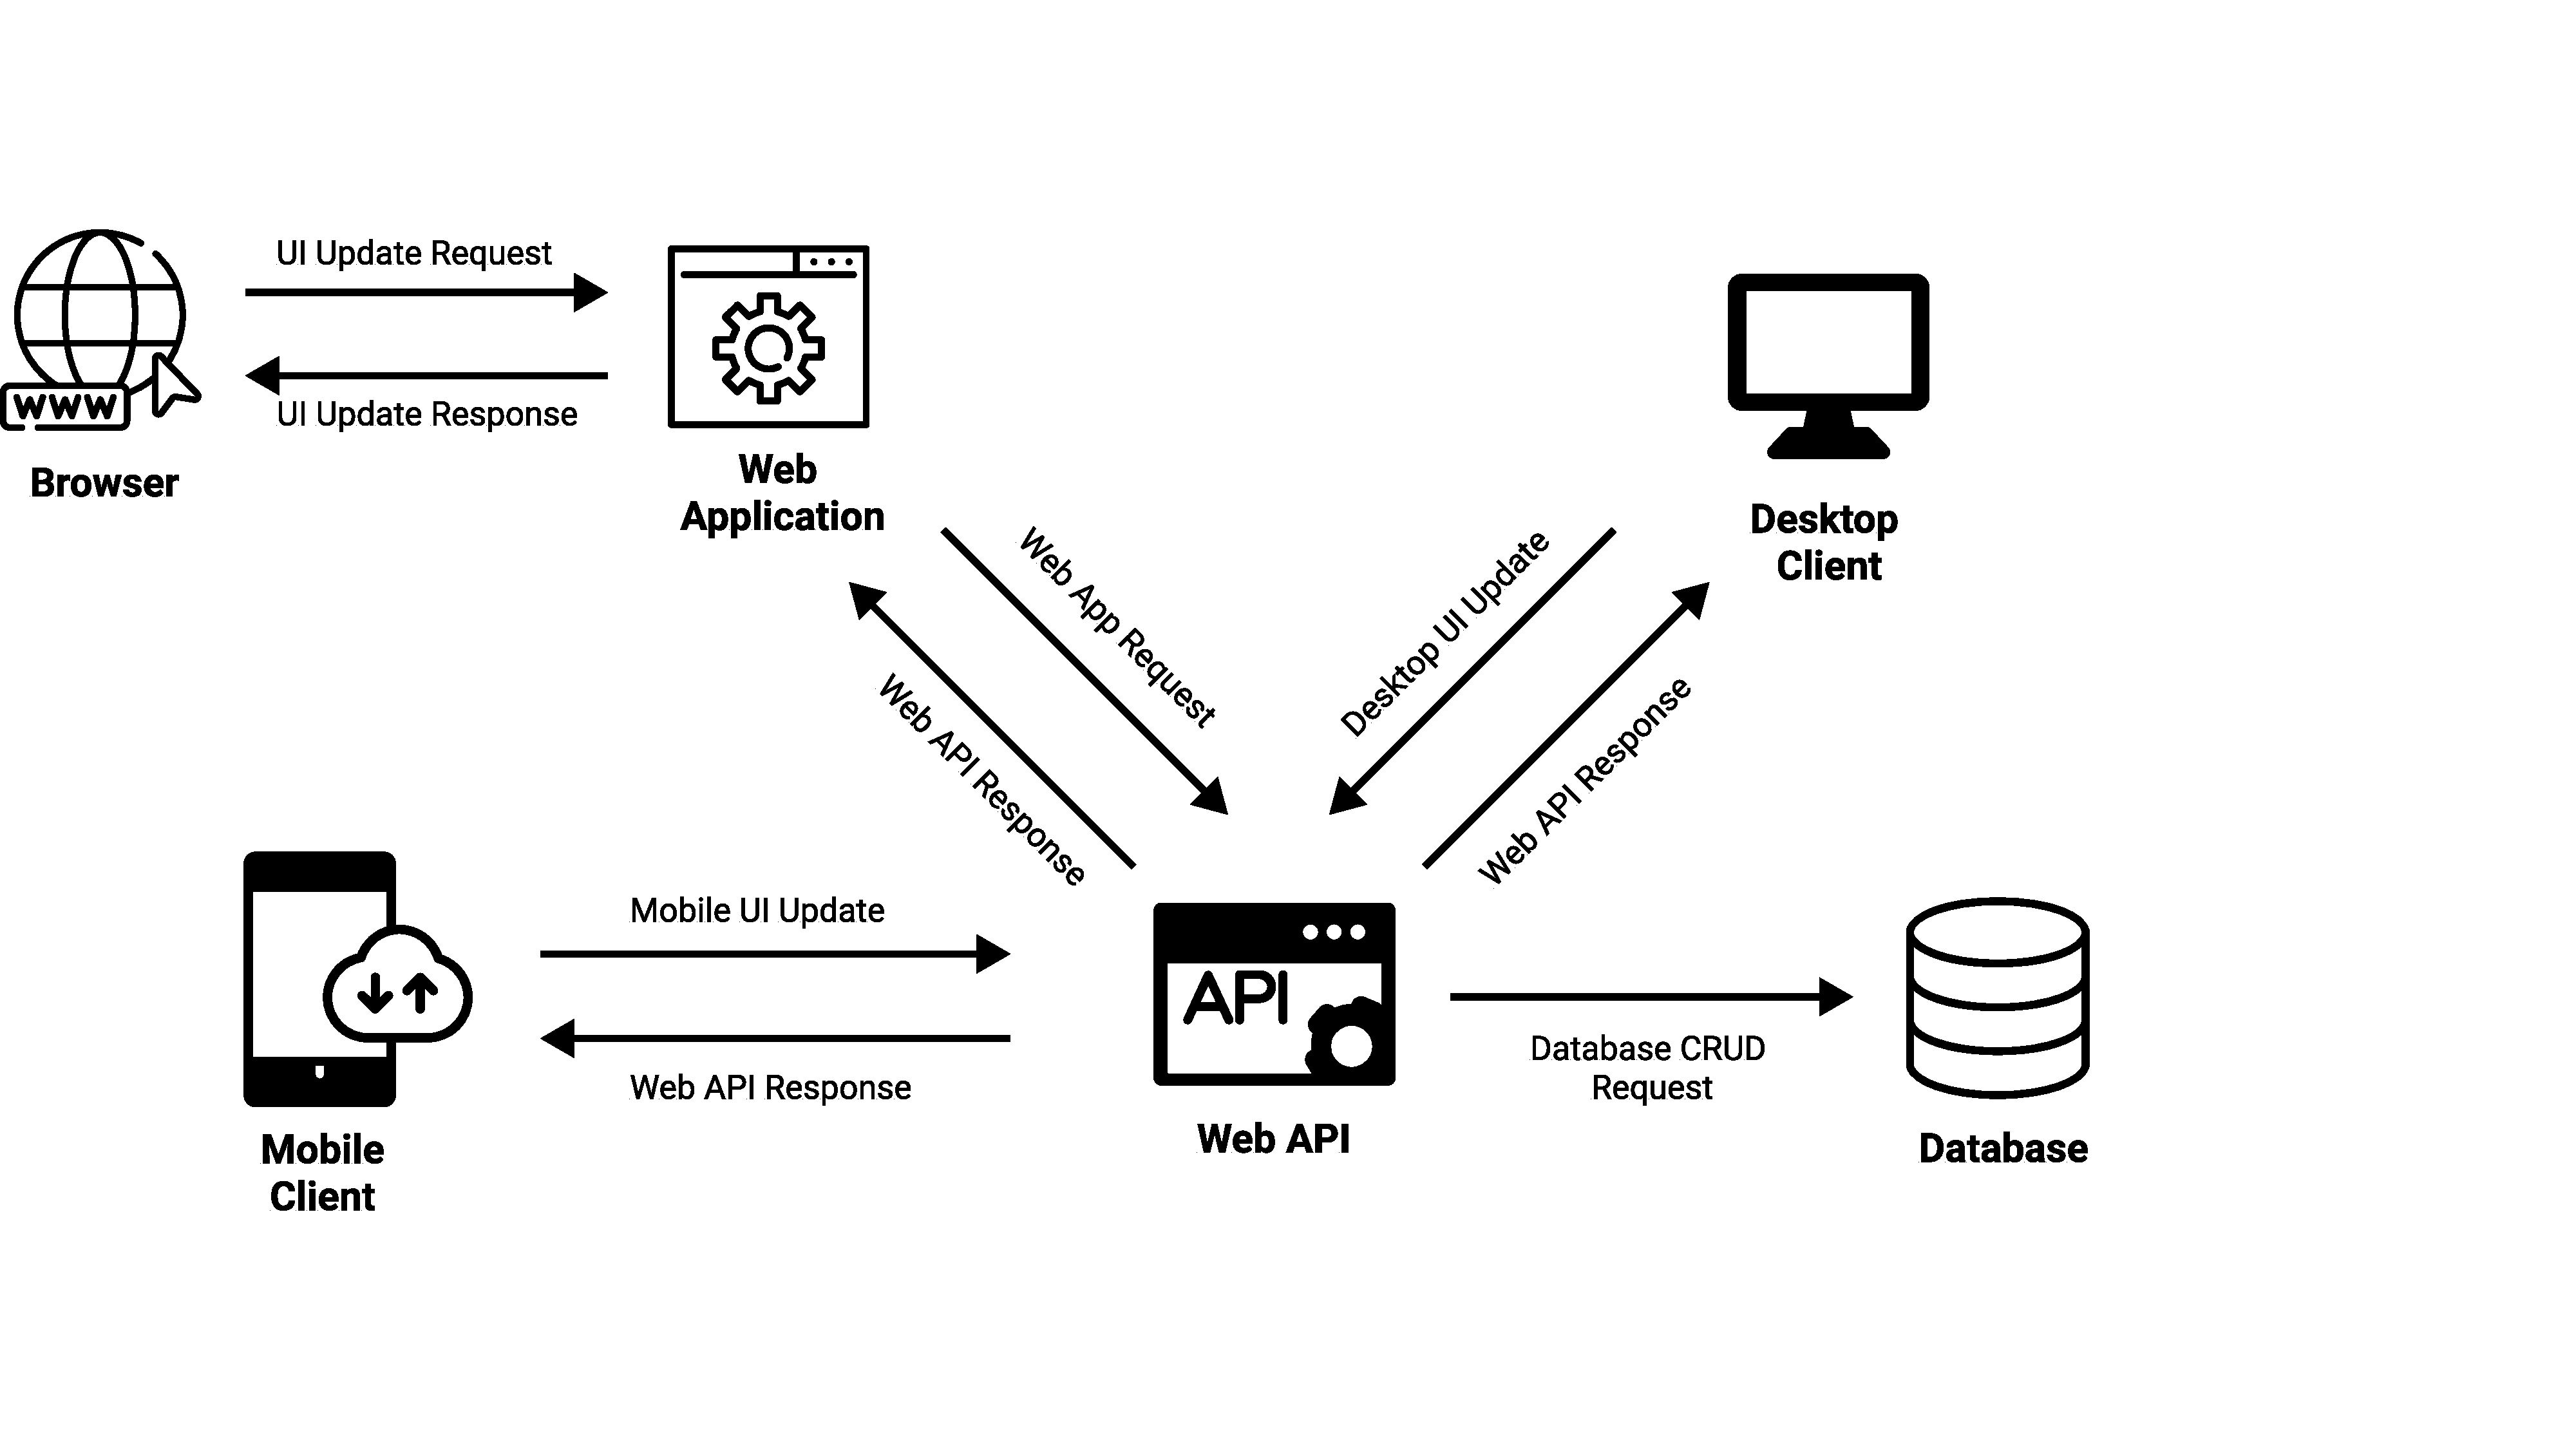
\includegraphics[width=1\textwidth]{Pictures/Threat_Modeling}
    \caption{Database diagram.}\label{fig:figure6}
\end{figure}

Hence, communication between software components is organised as follows\\

\textit{Browser - Web Application - Web API - Database communication model}
\begin{itemize}
    \item Browser downloads application static files from Web Application server.
    \item Browser sends a request to Web API\@.
    \item Web API checks access rights, executes business logic referring to the Database.
    \item Web API responds to the Browser.
    \item Browser user interface is being updated.
\end{itemize}

\textit{Desktop Client - Web API - Database communication model}
\begin{itemize}
    \item Desktop Client sends a request to update the user interface.
    \item Web API checks access rights, executes business logic referring to the Database.
    \item Web API responds to Desktop Client.
    \item Desktop Client's user interface updated as per response from the Web API\@.
\end{itemize}

\textit{Mobile Client - Web API - Database communication model}
\begin{itemize}
    \item Mobile Client sends a request to update the user interface.
    \item Web API checks access rights, executes business logic referring to the Database.
    \item Web API responds to the desktop Mobile Client.
    \item Mobile Client's user interface updated as per response from the Web API\@.
\end{itemize}

However, such communication models are under possible security vulnerabilities.
The first vulnerability that comes to mind is phishing.
An attacker could launch his own web application consuming our web API, therefore it is possible to log user actions
and get access to personal data or credentials.
Phishing attack could be mitigated using a properly configured Cross-Origin Resource Sharing policy that will restrict
the queries from the domains that do not meet the policy.
Like, for instance, it is done in our project

\begin{spverbatim}
    public static void Configure(
    IApplicationBuilder app,
    IWebHostEnvironment env)
    {
        ...

        app.UseCors(CorsPolicy);

        ...
    }

    public void ConfigureServices(IServiceCollection services)
    {
        ...

        services.AddCors(options =>
        {
            options.AddPolicy(CorsPolicy, builder =>
            {
                var allowedOrigins = Configuration
                        .GetSection("AllowedOrigins")
                        .Get<string[]>();

                builder.WithOrigins(allowedOrigins)
                       .AllowAnyMethod()
                       .AllowCredentials()
                       .AllowAnyHeader();
            });
        });

        ...
    }
\end{spverbatim}

The next potential vulnerability is improper TLS / SSL certificate configuration or usage of self-signed certificate,
to eliminate the vulnerability of the improper TLS certificate, it is recommended to follow the instructions and
\href{https://www.ssl.com/guide/ssl-best-practices/}{best practices}.

In addition, a potential vulnerability lies in the possibility of SQL injection.
The SQL injection vulnerability is eliminated by using parameters in string literals of the SQL query.
Also, it is necessary to pay attention to the configuration used ORM\@.

There is another danger that attacker may receive information about the application infrastructure through the error messages in the
response from the server, thus, it is recommended to use the unified \href{https://datatracker.ietf.org/doc/html/rfc7231}{response format}
from the server, which, in case of an error, will not contain the details of the error.

In order to provide proper authorization, it is recommended to use the roles for users in order to restrict an unauthorized
access to the resources available only to administrators.

The last but not least possible vulnerability -- is a famous worm and virus spreading problem.
Obviously, it is not a problem to get rid of the worms in local network with just a few devices connected,
however worms are really dangerous for the huge networks, like messenger considered to be.
The fight against the worms generally dependent on the end-user's security best practices education (at least user should
not use the public unprotected wi-fi networks) and firewall settings of the network.
However, the spread of viruses may be mitigated by the certain validation rules upon file upload, like for instance
\begin{spverbatim}
    public UploadDocumentCommandValidator()
    {
        var allowedExtensions = new List<string>
        {
            "jpg", "JPG", "txt", "TXT", "pdf",
            "PDF", "gif", "GIF", "png", "PNG"
        };

        RuleFor(x => x.FormFile).NotEmpty();

        RuleFor(x => x.FormFile.Length)
            .LessThanOrEqualTo(10 * 1024 * 1024);

        RuleFor(x => x.FormFile.FileName)
            .Cascade(CascadeMode.Stop)
            .NotEmpty()
            .Must(t =>
            {
                var validExtension = t.Split('.').Last();
                return allowedExtensions
                .Contains(validExtension);
            }).Length(1, 20);
    }
\end{spverbatim}

%\begin{enumerate}
%    \item \textbf{Browser UI Update Request}
%    \begin{itemize}
%        \item \textbf{Treat 1.1.} An adversary can perform action on behalf of other user due to lack of controls
%        against cross domain requests.
%        \item \textbf{Treat 1.5.} An adversary can spoof the target web application due to insecure TLS certificate configuration.
%        \item \textbf{Treat 1.8.} An adversary can gain access to sensitive data by performing SQL injection through Web App.
%        \item \textbf{Treat 1.10.} An adversary can deface the target web application by injecting malicious code or uploading dangerous files.
%        \item \textbf{Treat 1.11.} An adversary may spoof Desktop Web Browser (Chrome) and gain access to Web Application.
%        \item \textbf{Treat 1.12.} An adversary can create a fake website and launch phishing attacks.
%        \item \textbf{Treat 1.18.} An adversary can gain access to sensitive information through error messages.
%        \item \textbf{Treat 1.19.} An adversary can gain access to sensitive data by sniffing traffic to Web Application.
%    \end{itemize}
%    \item \textbf{Web App Request}
%    \begin{itemize}
%        \item \textbf{Treat 2.1.} An adversary may gain unauthorized access to Web API due to poor access control checks.
%        \item \textbf{Treat 2.2.} An adversary can gain access to sensitive information from an API through error messages.
%        \item \textbf{Treat 2.3.} An adversary can gain access to sensitive data by sniffing traffic to Web API\@.
%        \item \textbf{Treat 2.5.} Attacker can deny a malicious act on an API leading to repudiation issues.
%        \item \textbf{Treat 2.6.} An adversary may spoof Mango Web Application and gain access to Web API\@.
%        \item \textbf{Treat 2.7.} An adversary may inject malicious inputs into an API and affect downstream processes.
%        \item \textbf{Treat 2.8.} An adversary can gain access to sensitive data by performing SQL injection through Web API\@.
%    \end{itemize}
%    \item \textbf{Web API Response}
%    \begin{itemize}
%        \item \textbf{Treat 3.3.} An adversary can gain access to sensitive information through error messages.
%        \item \textbf{Treat 3.5.} An adversary can spoof the target web application due to insecure TLS certificate configuration.
%        \item \textbf{Treat 3.6.} An adversary can steal sensitive data like user credentials.
%        \item \textbf{Treat 3.7.} An adversary can create a fake website and launch phishing attacks.
%    \end{itemize}
%    \item \textbf{CRUD Request}
%    \begin{itemize}
%        \item \textbf{Treat 4.1.} An adversary can gain unauthorized access to database due to loose authorization rules.
%        \item \textbf{Treat 4.2.} An adversary can gain access to sensitive PII or HBI data in database.
%        \item \textbf{Treat 4.3.} An adversary can gain access to sensitive data by performing SQL injection.
%        \item \textbf{Treat 4.4.} An adversary can deny actions on database due to lack of auditing.
%        \item \textbf{Treat 4.5.} An adversary can tamper critical database securables and deny the action.
%        \item \textbf{Treat 4.7.} An adversary can gain unauthorized access to database due to lack of network access protection.
%    \end{itemize}
%    \item \textbf{Mobile UI Update}
%    \begin{itemize}
%        \item \textbf{Treat 5.1.} An adversary can gain access to sensitive data by performing SQL injection through Web API.
%        \item \textbf{Treat 5.2.} An adversary can reverse engineer and tamper binaries.
%        \item \textbf{Treat 5.3.} An adversary may inject malicious inputs into an API and affect downstream processes.
%        \item \textbf{Treat 5.4.} An adversary may spoof Mobile App (IOS, Android) and gain access to Web API\@.
%        \item \textbf{Treat 5.5.} An adversary obtains refresh or access tokens from Mobile App (IOS, Android) and uses them to
%        obtain access to the Mango Web API\@.
%        \item \textbf{Treat 5.6.} Attacker can deny a malicious act on an API leading to repudiation issues.
%        \item \textbf{Treat 5.7.} An adversary can gain access to sensitive data stored in Web API's config files.
%        \item \textbf{Treat 5.8.} An adversary can gain sensitive data from mobile device.
%        \item \textbf{Treat 5.9.} An adversary can gain access to sensitive data by sniffing traffic to Web API\@.
%        \item \textbf{Treat 5.10.} An adversary can gain access to sensitive data by sniffing traffic from Mobile client.
%        \item \textbf{Treat 5.11.} An adversary can gain access to sensitive information from an API through error messages.
%        \item \textbf{Treat 5.12.} An adversary may gain unauthorized access to Web API due to poor access control checks.
%        \item \textbf{Treat 5.13.} An adversary may jail break into a mobile device and gain elevated privilege.
%    \end{itemize}
%\end{enumerate}